For this part we used a pair of images to attempt image stitching using SIFT and homography computed using the RANSAC algorithm. Starting with extracting SIFT features, we used sorted matches (sorted according to the Euclidean distance) to comput homography from the left image to the right image. The keypoint matches yielded are shown in Fig.~\ref{fig:lionMatches}.

\begin{figure}[ht]
\centering
	\begin{subfigure}{0.4\textwidth}
    {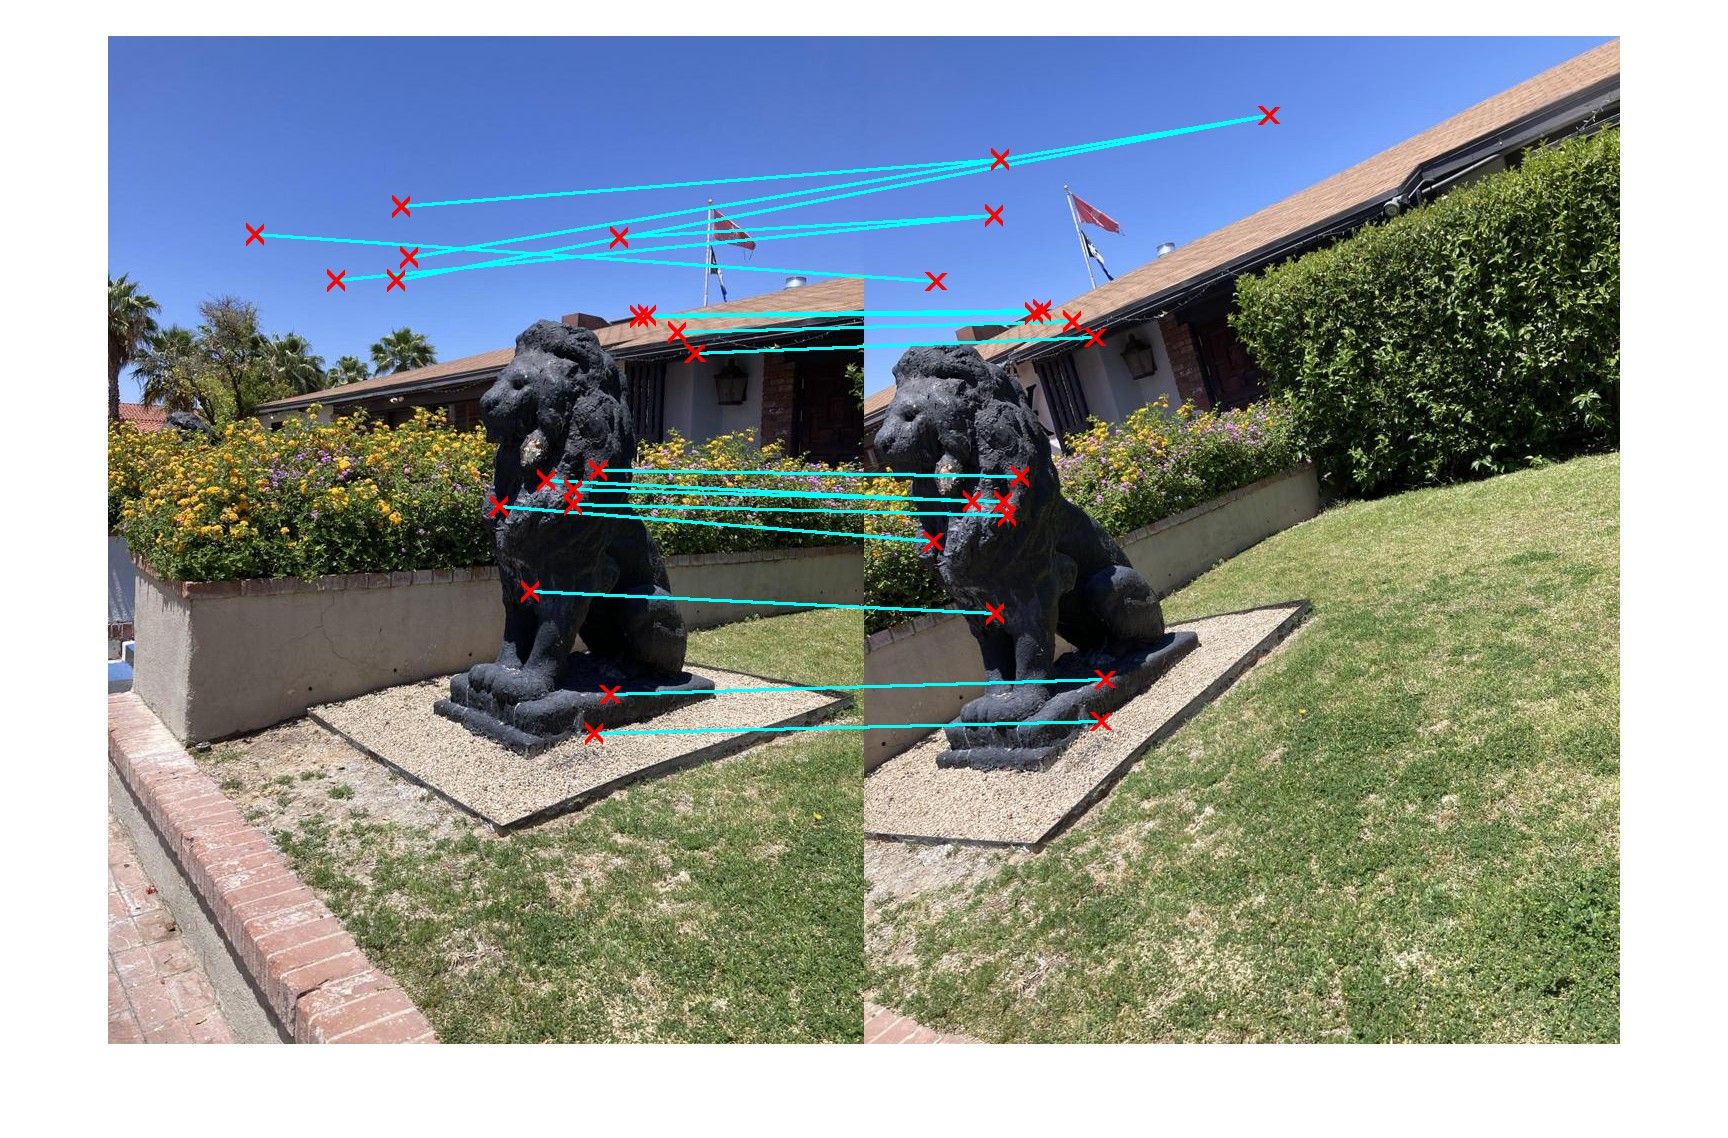
\includegraphics[width=3in]{new_figs/lion_siftFeats20.jpg}}
	\caption{20 keypoint matches}
	\end{subfigure}
	\begin{subfigure}{0.4\textwidth}
    {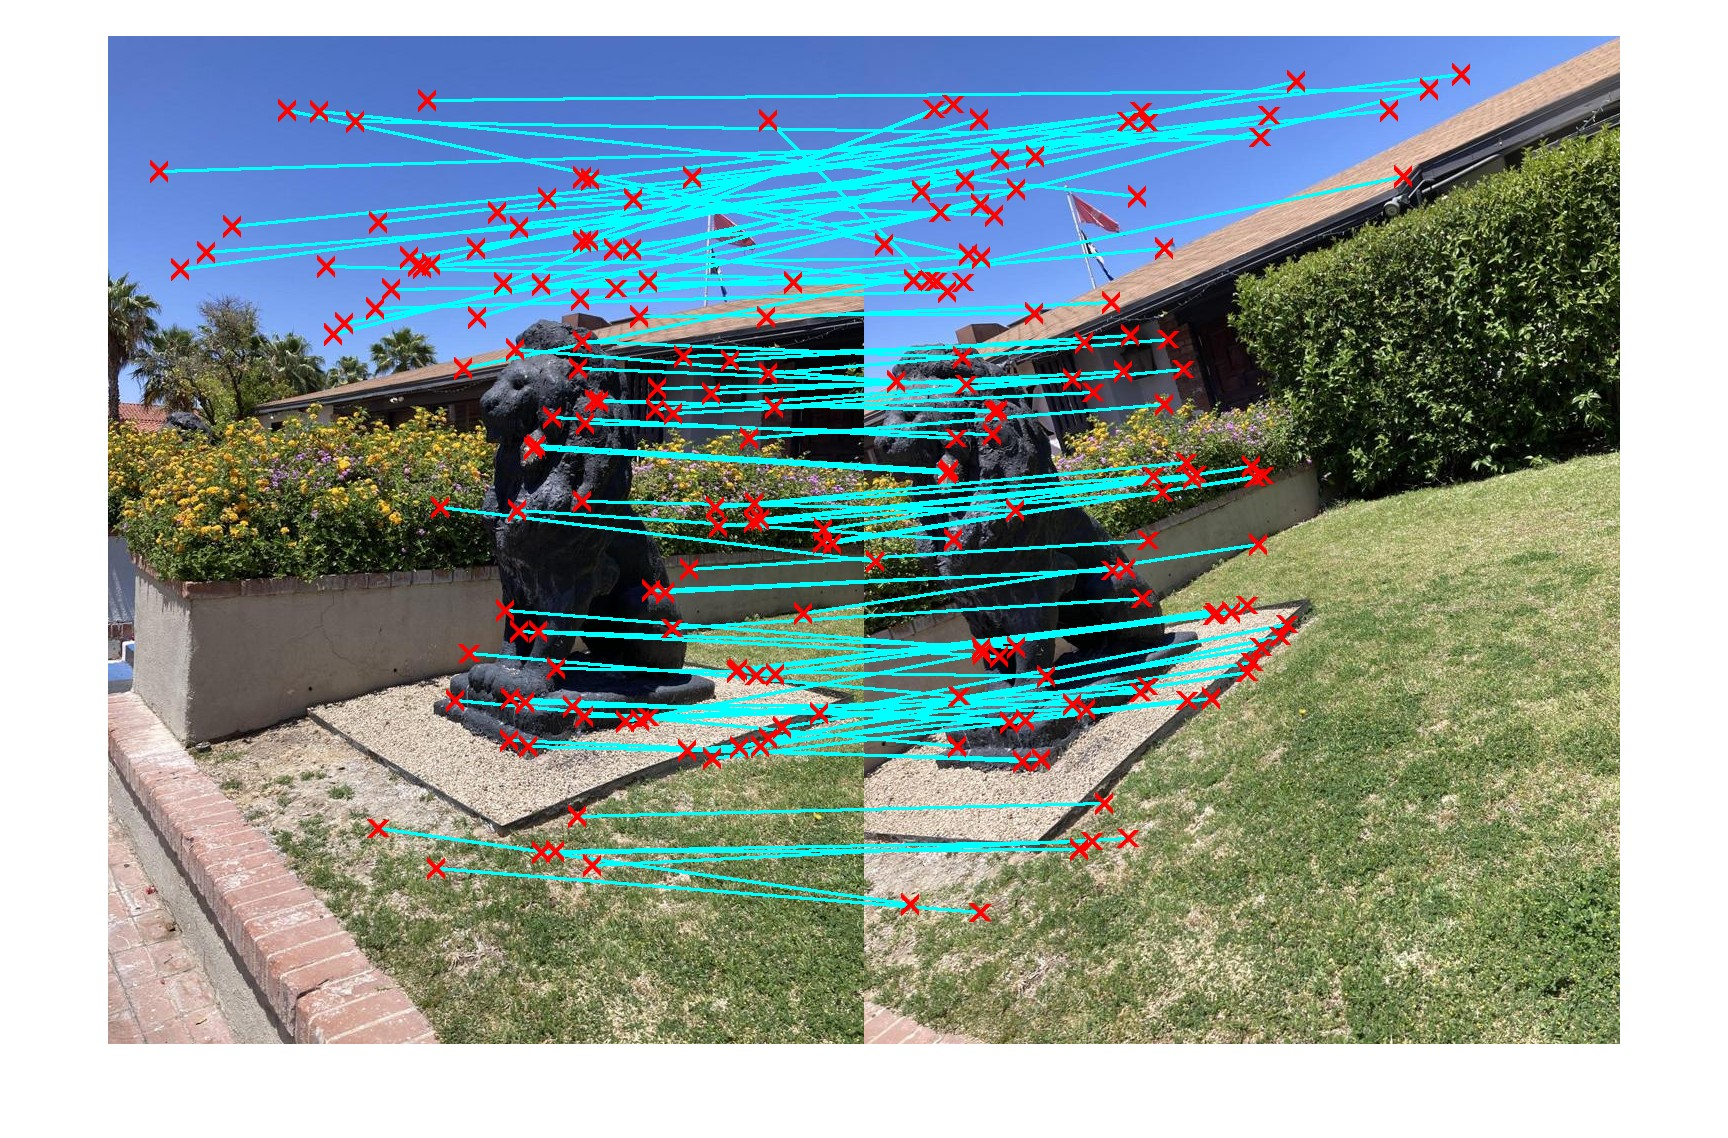
\includegraphics[width=3in]{new_figs/lion_siftFeats108.jpg}
	\caption{108 keypoint matches}
	\end{subfigure}
	\caption{Figure showing keypoint matches across two views of the same scene. These matches were extracted for image stitching. }
\label{fig:lionMatches}
\end{figure}

We then created a white RGB image to hold two images together in a stitch and fixed the position for the left image. Then for each pixel in the right image, we estimated the mappting of the pixel locations in the stitch using the homography computed using the RANSAC algorithm. We faced some trouble getting the stitch correctly. Fig.~\ref{fig:lionStich} shows the example of output we received. Conceptually, it made sense of what we were trying to achieve (mapping the points in the second image on top of the first image using the homography -- as homography tells us the geometric transformation from one image to another). Most of our "stitched" results looked like they require rotation and translation but from class lectures, we grasped that homography takes care of rotation and translation, so we weren't sure of what exactly was going awry. It also looked like the second image was being mapped as sheered. I looked into the imwarp function on MATLAB, but wasn't sure if that was the correct route to take. The other challenge we faced is that while mapping, some points were exploding or splitting from the middle, this can be observed in images (c), (d), and (f) of Fig.~\ref{fig:lionStich}. The mapping looks funny for most, we believe this happened solely in the step where we computed mapping points using homography found from RANSAC. From results of previous parts of the assignment, we believe that our DLT method and RANSAC algorithm were performing correctly, so it was hard to debug here what's going wrong.

\begin{figure}[ht]
\centering
	\begin{subfigure}{0.4\textwidth}
    {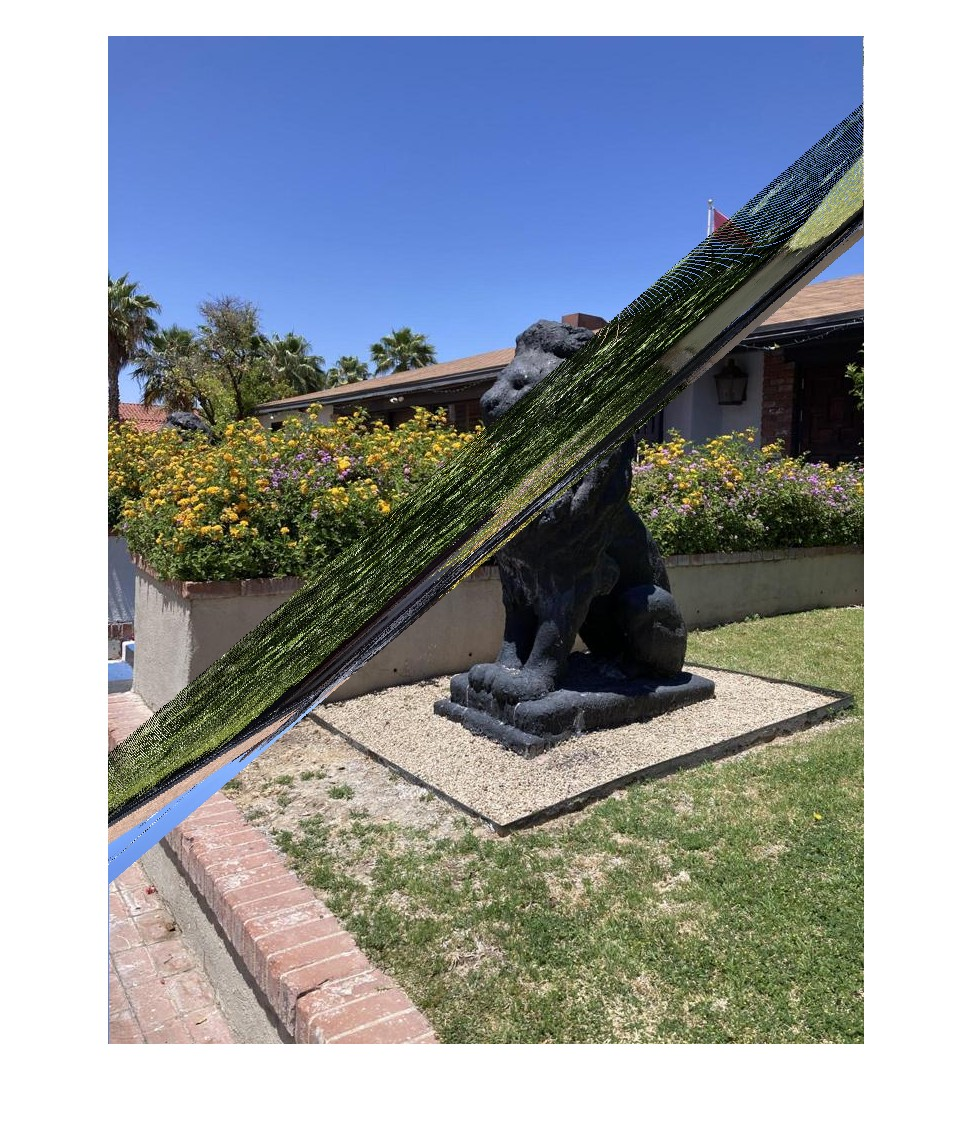
\includegraphics[width=2.5in]{new_figs/1_stitch.jpg}}
	\caption{}
	\end{subfigure}
	\begin{subfigure}{0.4\textwidth}
    {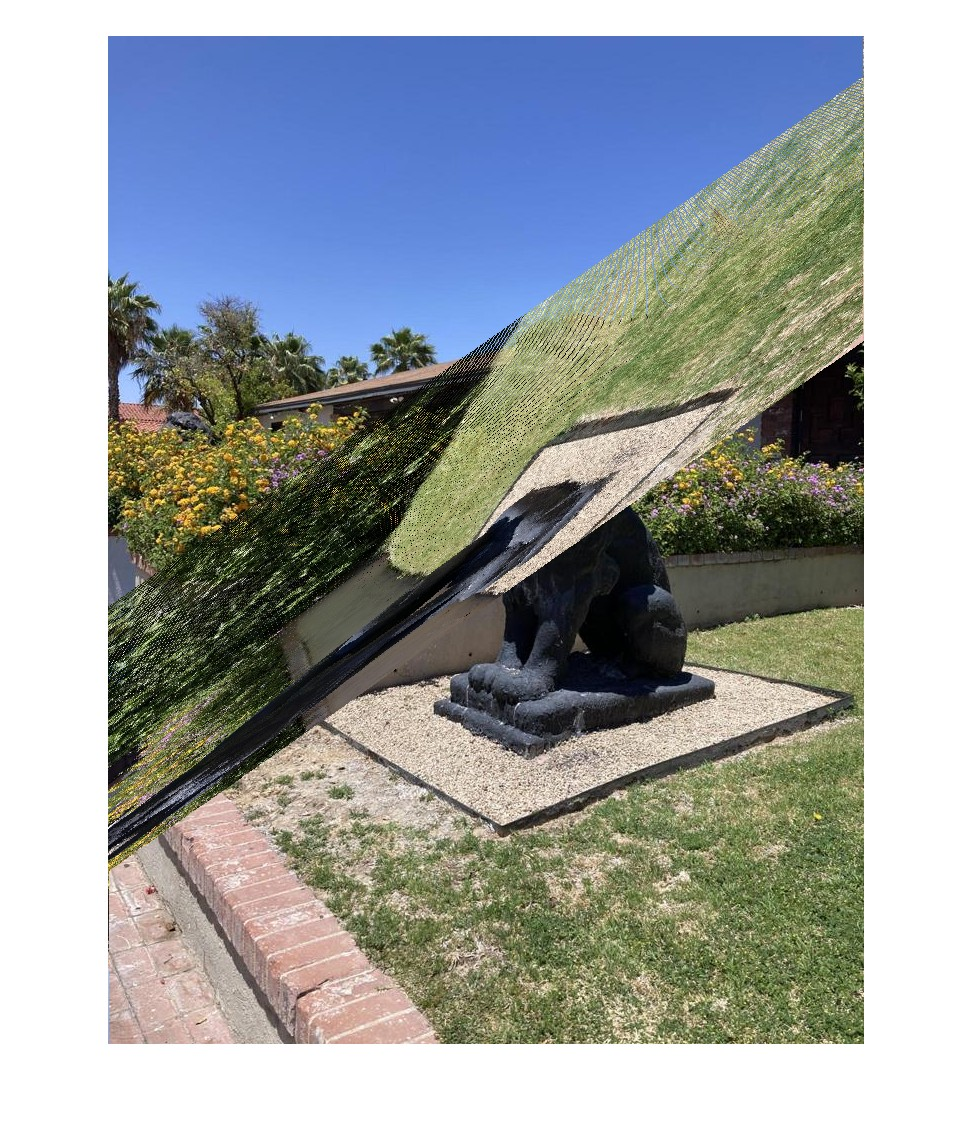
\includegraphics[width=2.5in]{new_figs/2_stitch.jpg}
	\caption{}
	\end{subfigure}
	\begin{subfigure}{0.4\textwidth}
    {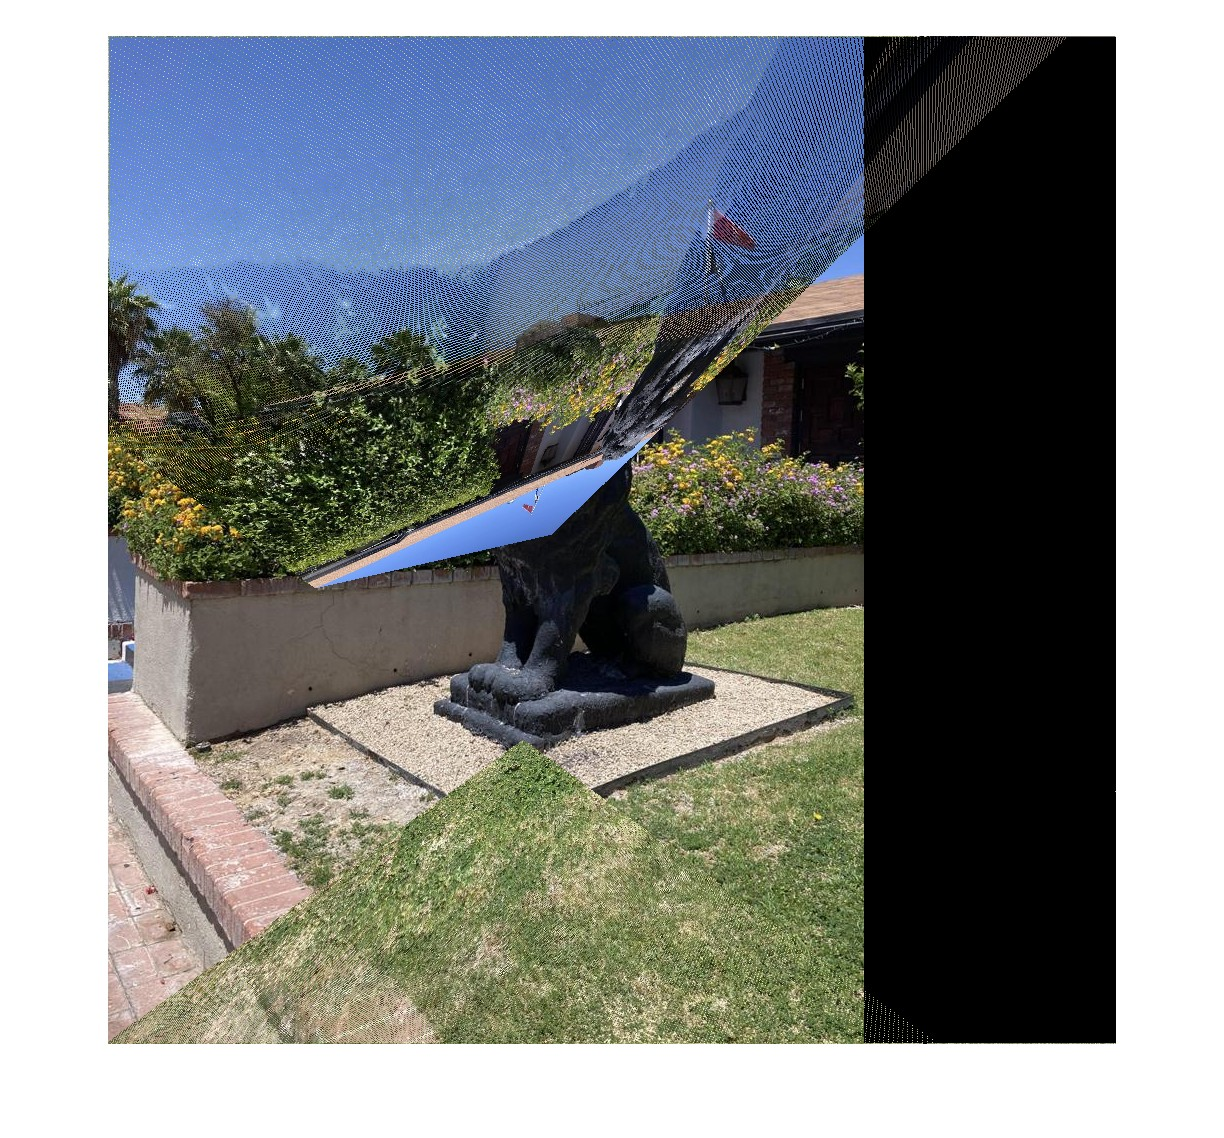
\includegraphics[width=2.5in]{new_figs/3_stitch.jpg}}
	\caption{}
	\end{subfigure}
	\begin{subfigure}{0.4\textwidth}
    {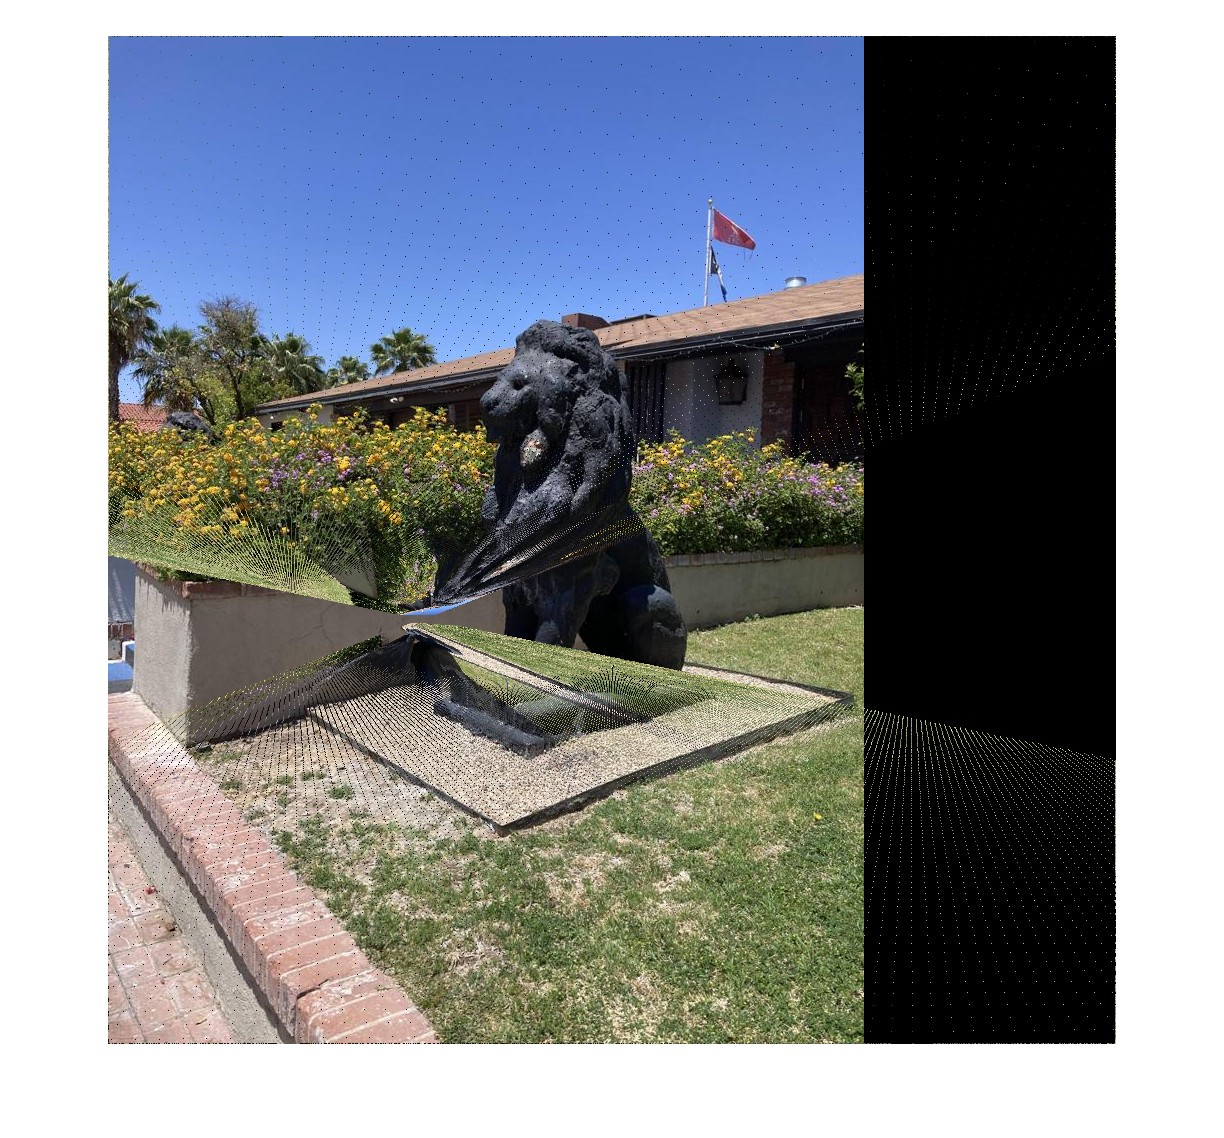
\includegraphics[width=2.5in]{new_figs/4_stitch.jpg}
	\caption{}
	\end{subfigure}
	\begin{subfigure}{0.4\textwidth}
    {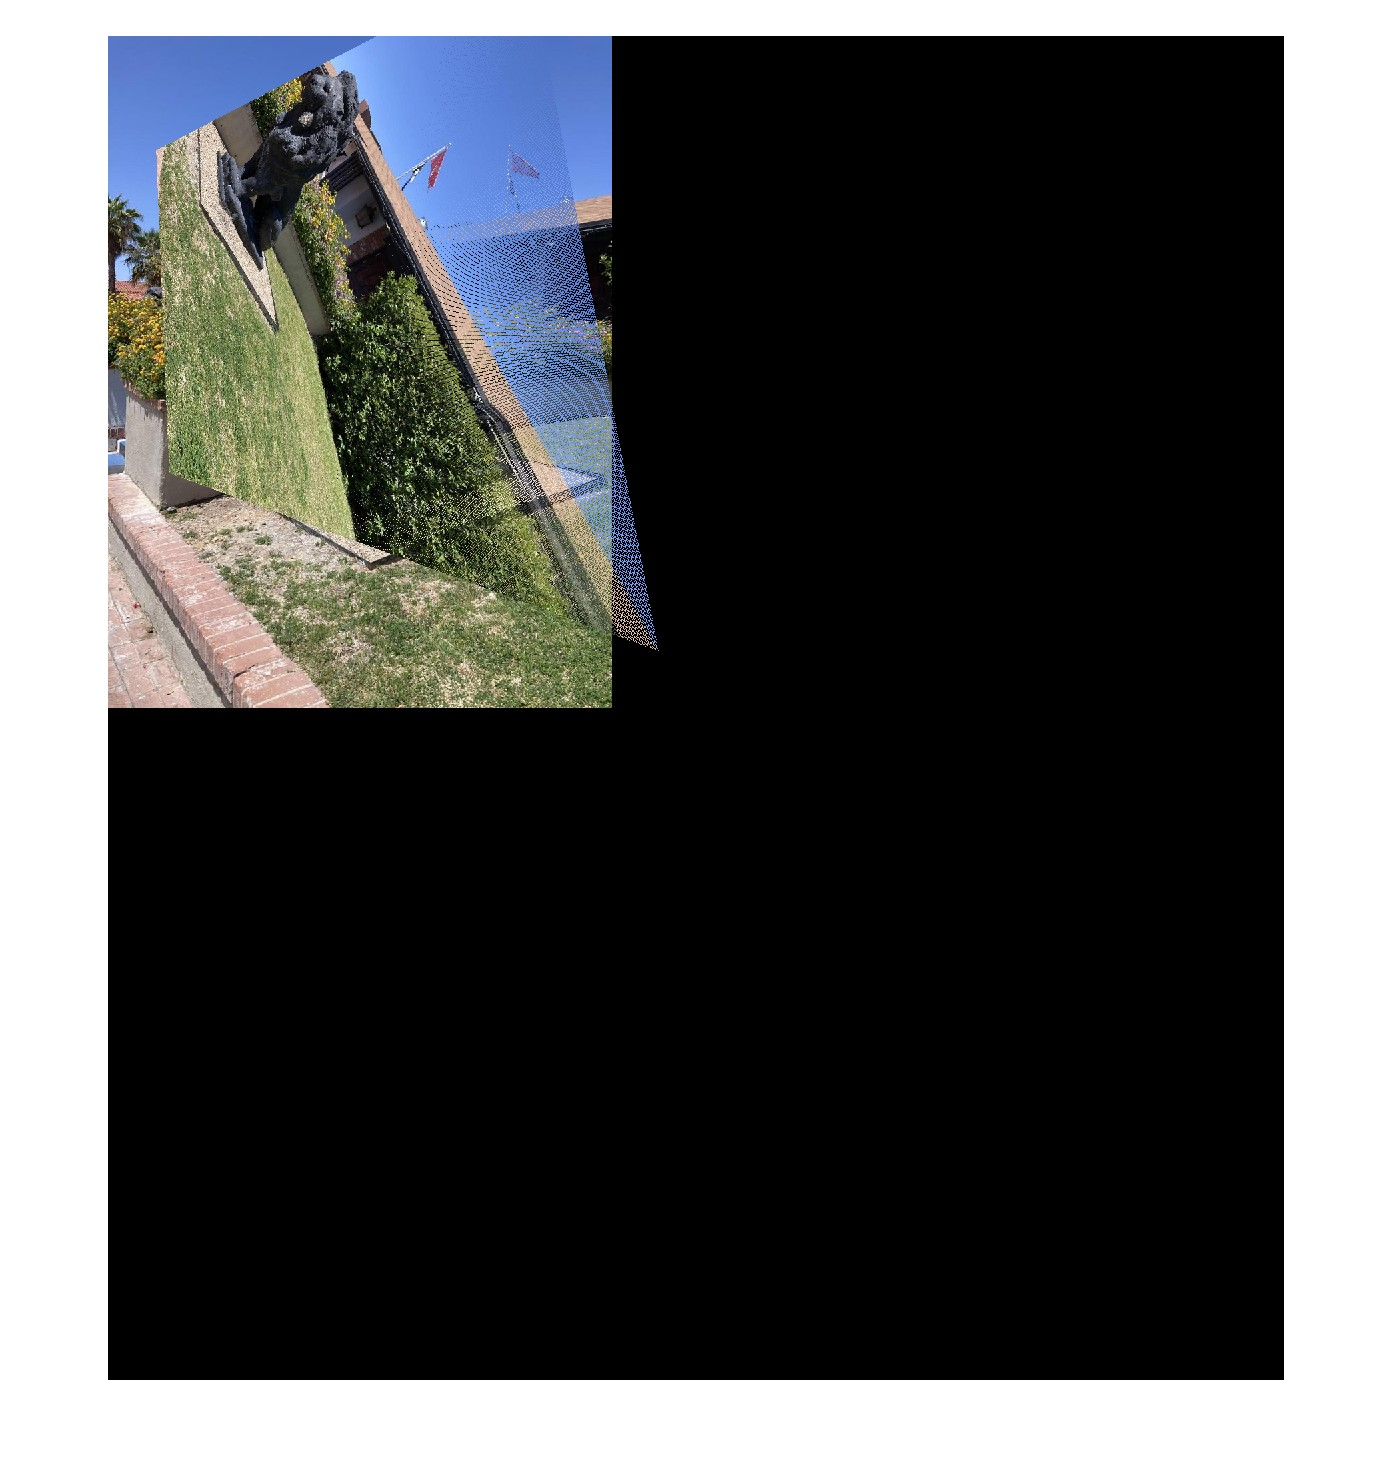
\includegraphics[width=2.5in]{new_figs/5_stitch.jpg}}
	\caption{}
	\end{subfigure}
	\begin{subfigure}{0.4\textwidth}
    {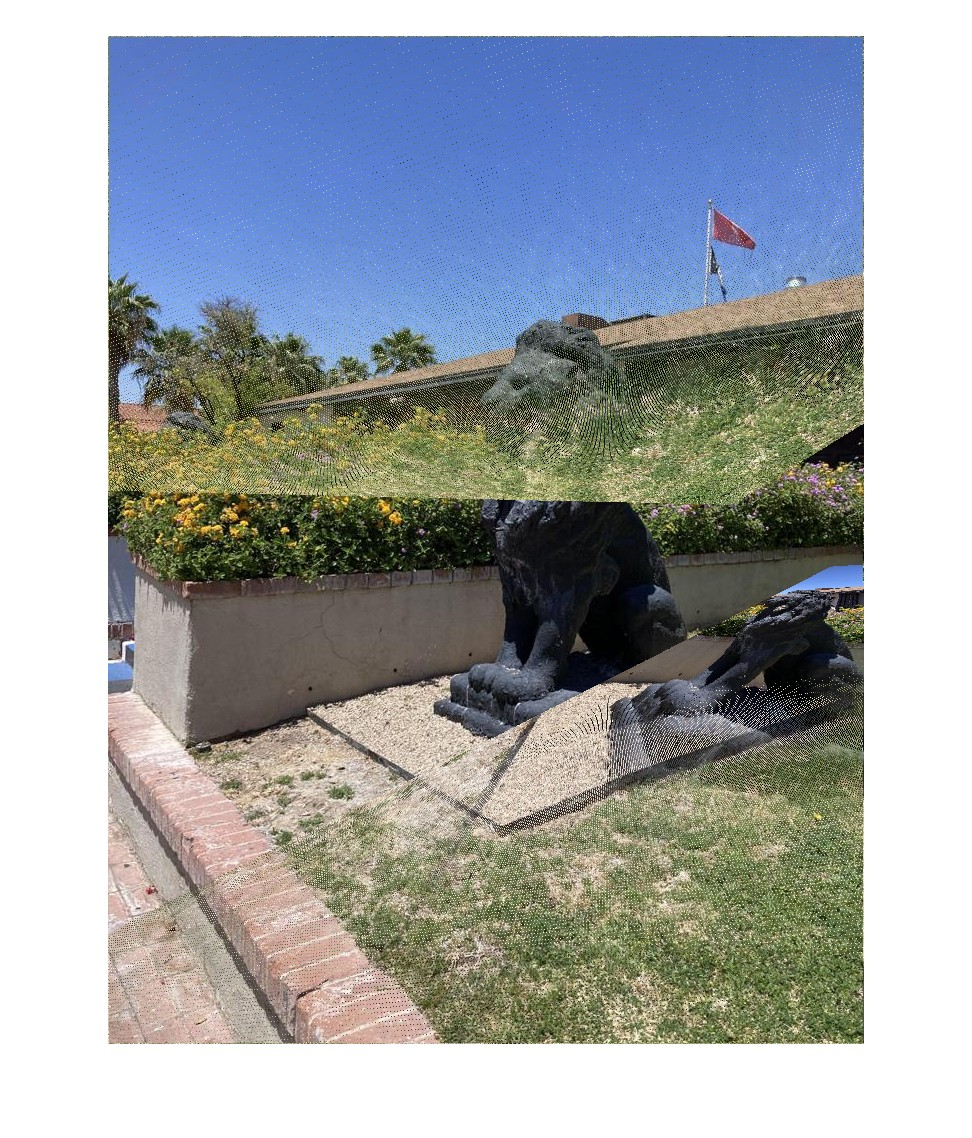
\includegraphics[width=2.5in]{new_figs/6_stitch.jpg}
	\caption{}
	\end{subfigure}
	\caption{Figure showing results from attempted image stitching. Please see text on the previous page for more details regarding these images.}
\label{fig:lionStich}
\end{figure}
